\documentclass[tikz]{standalone}

%graphics
\usepackage{xcolor}

\usetikzlibrary{shapes.geometric, shapes.multipart, arrows, calc, through}


\colorlet{dot-color}{black!80}
\def\cellsize{0.425}
\tikzset{
  pics/gcell/.style = {
    code = {
      \coordinate (-center) at (0,0);
      
      \fill +(-0.45,-0.45) coordinate(-sw) 
      -- +(-0.45, 0.45) coordinate(-nw)
      -- +( 0.45, 0.45) coordinate(-ne)
      -- +( 0.45,-0.45) coordinate(-se)
      -- cycle;
      \coordinate (-swo) at ($ (-center)!0.5!(-sw) $);
      \coordinate (-nwo) at ($ (-center)!0.5!(-nw) $);
      \coordinate (-neo) at ($ (-center)!0.5!(-ne) $);
      \coordinate (-seo) at ($ (-center)!0.5!(-se) $);
      
      \coordinate (-south) at ($ (-sw)!.5!(-se) $);
      \coordinate (-north) at ($ (-nw)!.5!(-ne) $);
      \coordinate (-west)  at ($ (-sw)!.5!(-nw) $);
      \coordinate (-east)  at ($ (-se)!.5!(-ne) $);
      
      \fill[white] (-swo) let \p1=($ (-center)!.5!(-swo) $) in circle ({veclen(\x1,\y1)});
      \fill[white] (-nwo) let \p1=($ (-center)!.5!(-nwo) $) in circle ({veclen(\x1,\y1)});
      \fill[white] (-neo) let \p1=($ (-center)!.5!(-neo) $) in circle ({veclen(\x1,\y1)});
      \fill[white] (-seo) let \p1=($ (-center)!.5!(-seo) $) in circle ({veclen(\x1,\y1)});
      
      \ifnum#1=1\relax
      \fill[dot-color] (-swo) let \p1=($ (-center)!.32!(-swo) $) in circle ({veclen(\x1,\y1)});
      \fill[dot-color] (-neo) let \p1=($ (-center)!.32!(-neo) $) in circle ({veclen(\x1,\y1)});
      \else
      \ifnum#1=-1\relax
      \fill[dot-color] (-nwo) let \p1=($ (-center)!.32!(-nwo) $) in circle ({veclen(\x1,\y1)});
      \fill[dot-color] (-seo) let \p1=($ (-center)!.32!(-seo) $) in circle ({veclen(\x1,\y1)});
      \else
      \fill[dot-color] (-swo) let \p1=($ (-center)!.22!(-swo) $) in circle ({veclen(\x1,\y1)});
      \fill[dot-color] (-nwo) let \p1=($ (-center)!.22!(-nwo) $) in circle ({veclen(\x1,\y1)});
      \fill[dot-color] (-neo) let \p1=($ (-center)!.22!(-neo) $) in circle ({veclen(\x1,\y1)});
      \fill[dot-color] (-seo) let \p1=($ (-center)!.22!(-seo) $) in circle ({veclen(\x1,\y1)});
      \fi
      \fi
    }
  },
  pics/gcell/.default={0},
  pics/gcross_cell/.style = {
    code = {%
      \coordinate (-center) at (0,0);
      \fill +(-0.45,-0.45) coordinate(-sw) 
      -- +(-0.45, 0.45) coordinate(-nw)
      -- +( 0.45, 0.45) coordinate(-ne)
      -- +( 0.45,-0.45) coordinate(-se)
      -- cycle;
      \coordinate (-north) at ($(-ne)!0.5!(-nw)$);
      \coordinate (-south) at ($(-se)!0.5!(-sw)$);
      \coordinate (-east) at ($(-ne)!0.5!(-se)$);
      \coordinate (-west) at ($(-nw)!0.5!(-sw)$);
      
      \coordinate (-no) at ($(-center)!0.65!(-north)$);
      \coordinate (-so) at ($(-center)!0.65!(-south)$);
      \coordinate (-eo) at ($(-center)!0.65!(-east)$);
      \coordinate (-wo) at ($(-center)!0.65!(-west)$);
      
      \fill[white] (-no) let \p1=($ (-center)!0.5!(-no) $) in circle ({veclen(\x1,\y1)});
      \fill[white] (-so) let \p1=($ (-center)!0.5!(-so) $) in circle ({veclen(\x1,\y1)});
      \fill[white] (-eo) let \p1=($ (-center)!0.5!(-eo) $) in circle ({veclen(\x1,\y1)});
      \fill[white] (-wo) let \p1=($ (-center)!0.5!(-wo) $) in circle ({veclen(\x1,\y1)});
      
      \ifnum#1=1\relax
      \fill[dot-color] (-no) let \p1=($ (-center)!.32!(-no) $) in circle ({veclen(\x1,\y1)});
      \fill[dot-color] (-so) let \p1=($ (-center)!.32!(-so) $) in circle ({veclen(\x1,\y1)});
      \else
      \ifnum#1=-1\relax
      \fill[dot-color] (-eo) let \p1=($ (-center)!.32!(-eo) $) in circle ({veclen(\x1,\y1)});
      \fill[dot-color] (-wo) let \p1=($ (-center)!.32!(-wo) $) in circle ({veclen(\x1,\y1)});
      \fi
      \fi
    }
  },
  pics/cell/.style = {
    code = {%
      \coordinate (-center) at (0,0);
      \coordinate (-east) at (\cellsize, 0);
      \coordinate (-north) at (0, \cellsize);
      \coordinate (-west) at (-\cellsize, 0);
      \coordinate (-south) at (0, -\cellsize);
      
      \fill[draw=black, line width=0.2pt, rounded corners=0.3pt] (-west |- -south) rectangle (-east |- -north);
      \foreach \d in {-east, -north, -west, -south}
      \draw[black, line width=.2pt] ($(-center)!.7!45:(\d)$) circle[radius=.12];
    }
  },
  pics/via/.style={
    code={%
      \coordinate (-center) at (0,0);
      \coordinate (-east) at (\cellsize, 0);
      \coordinate (-north) at (0, \cellsize);
      \coordinate (-west) at (-\cellsize, 0);
      \coordinate (-south) at (0, -\cellsize);
      
      \fill[draw=black, line width=0.2pt, rounded corners=0.3pt] (-west |- -south) rectangle (-east |- -north);
      \draw[black, line width=0.2pt] (-center) circle [radius=0.32];
    }
  },
  pics/crossline/.style={
    code={%
      \coordinate (-center) at (0,0);
      \coordinate (-east) at (\cellsize, 0);
      \coordinate (-north) at (0, \cellsize);
      \coordinate (-west) at (-\cellsize, 0);
      \coordinate (-south) at (0, -\cellsize);
      
      \fill[draw=black, line width=0.2pt, rounded corners=0.3pt] (-west |- -south) rectangle (-east |- -north);
      \foreach \d in {-east, -north, -west, -south}
      \draw[black, line width=.2pt] (-center) -- ($(-center)!.9!45:(\d)$);
    }
  },
  pics/fixed/.style={
    code={%
      \coordinate (-center) at (0,0);
      \coordinate (-east) at (\cellsize, 0);
      \coordinate (-north) at (0, \cellsize);
      \coordinate (-west) at (-\cellsize, 0);
      \coordinate (-south) at (0, -\cellsize);
      
      \fill[draw=black, line width=0.2pt, rounded corners=0.3pt] (-west |- -south) rectangle (-east |- -north);
      \ifnum#1=0\relax
      \foreach \d in {-north, -south}
      \filldraw[white, line width=.2pt] ($(-center)!.7!45:(\d)$) circle[radius=.12];
      \else
      \foreach \d in {-east, -west}
      \filldraw[white, line width=.2pt] ($(-center)!.7!45:(\d)$) circle[radius=.12];
      \fi
    }
  },
}
\definecolor{clock0}{HTML}{86E291}
\definecolor{clock1}{HTML}{FFA5FA}
\definecolor{clock2}{HTML}{00C8BC}
\definecolor{clock3}{HTML}{F2F2F2}
\definecolor{input}{HTML}{008DC8}
\definecolor{output}{HTML}{E28686}
\definecolor{fixed}{HTML}{000000}

\colorlet{cs0}{lightgray!20}
\colorlet{cs1}{lightgray!50}
\colorlet{cs2}{lightgray}
\colorlet{cs3}{gray}

%\definecolor{clock0}{RGB}{89,89,91}
%\definecolor{clock1}{RGB}{129,130,132}
%\definecolor{clock2}{RGB}{210,210,212}
%\definecolor{clock3}{RGB}{168,169,173}
%\definecolor{input}{RGB}{230,230,230}
%\definecolor{output}{RGB}{40,40,40}
%\definecolor{fixed}{HTML}{000000}

\definecolor{clock0}{RGB}{89,89,91}
\definecolor{clock1}{RGB}{129,130,132}
\definecolor{clock2}{RGB}{210,210,212}
\definecolor{clock3}{RGB}{168,169,173}
\definecolor{input}{RGB}{230,230,230}
\definecolor{output}{RGB}{40,40,40}
\definecolor{fixed}{HTML}{000000}




\begin{document}

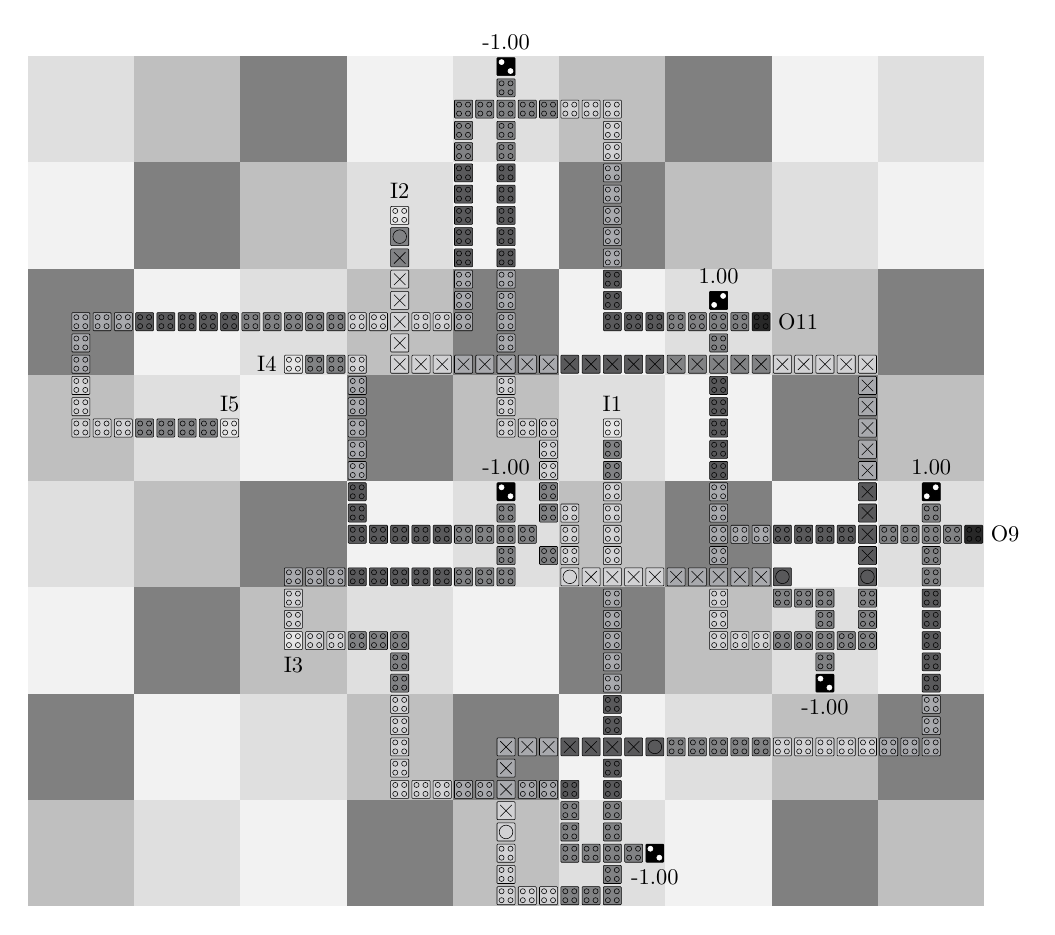
\begin{tikzpicture}[scale=0.27,transform shape]

\begin{scope}[
x=5cm,y=5cm,
shift={(0cm,-20cm)},
c0/.style={shape=rectangle, fill=cs0, text=black, minimum size=5cm},
c1/.style={shape=rectangle, fill=cs1, text=black, minimum size=5cm},
c2/.style={shape=rectangle, fill=cs2, text=black, minimum size=5cm},
c3/.style={shape=rectangle, fill=cs3, text=black, minimum size=5cm},
]
\node[c2] at (0,0) {};
\node[c1] at (1,0) {};
\node[c0] at (2,0) {};
\node[c3] at (3,0) {};
\node[c2] at (4,0) {};
\node[c1] at (5,0) {};
\node[c0] at (6,0) {};
\node[c3] at (7,0) {};
\node[c2] at (8,0) {};

\node[c3] at (0,1) {};
\node[c0] at (1,1) {};
\node[c1] at (2,1) {};
\node[c2] at (3,1) {};
\node[c3] at (4,1) {};
\node[c0] at (5,1) {};
\node[c1] at (6,1) {};
\node[c2] at (7,1) {};
\node[c3] at (8,1) {};

\node[c0] at (0,2) {};
\node[c3] at (1,2) {};
\node[c2] at (2,2) {};
\node[c1] at (3,2) {};
\node[c0] at (4,2) {};
\node[c3] at (5,2) {};
\node[c2] at (6,2) {};
\node[c1] at (7,2) {};
\node[c0] at (8,2) {};

\node[c1] at (0,3) {};
\node[c2] at (1,3) {};
\node[c3] at (2,3) {};
\node[c0] at (3,3) {};
\node[c1] at (4,3) {};
\node[c2] at (5,3) {};
\node[c3] at (6,3) {};
\node[c0] at (7,3) {};
\node[c1] at (8,3) {};

\node[c2] at (0,4) {};
\node[c1] at (1,4) {};
\node[c0] at (2,4) {};
\node[c3] at (3,4) {};
\node[c2] at (4,4) {};
\node[c1] at (5,4) {};
\node[c0] at (6,4) {};
\node[c3] at (7,4) {};
\node[c2] at (8,4) {};

\node[c3] at (0,5) {};
\node[c0] at (1,5) {};
\node[c1] at (2,5) {};
\node[c2] at (3,5) {};
\node[c3] at (4,5) {};
\node[c0] at (5,5) {};
\node[c1] at (6,5) {};
\node[c2] at (7,5) {};
\node[c3] at (8,5) {};

\node[c0] at (0,6) {};
\node[c3] at (1,6) {};
\node[c2] at (2,6) {};
\node[c1] at (3,6) {};
\node[c0] at (4,6) {};
\node[c3] at (5,6) {};
\node[c2] at (6,6) {};
\node[c1] at (7,6) {};
\node[c0] at (8,6) {};

\node[c1] at (0,7) {};
\node[c2] at (1,7) {};
\node[c3] at (2,7) {};
\node[c0] at (3,7) {};
\node[c1] at (4,7) {};
\node[c2] at (5,7) {};
\node[c3] at (6,7) {};
\node[c0] at (7,7) {};
\node[c1] at (8,7) {};
\end{scope}

\pic[clock2] at (0,0) {cell};
\pic[clock2] at (0,1) {cell};
\pic[clock2] at (0,2) {cell};
\pic[clock3] at (0,3) {cell};
\pic[clock3] at (0,4) {cell};
\pic[clock3] at (0,5) {cell};

\pic(3)[input] at (10,-10) {cell};
\node[below,scale=3] at (3-south) {I3};
\pic[clock2] at (10,-9) {cell};
\pic[clock2] at (10,-8) {cell};
\pic[clock3] at (10,-7) {cell};

\pic[clock0] at (13,-5) {cell};
\pic[clock0] at (13,-4) {cell};
\pic[clock0] at (13,-3) {cell};
\pic[clock3] at (13,-2) {cell};
\pic[clock3] at (13,-1) {cell};
\pic[clock3] at (13,0) {cell};
\pic[clock3] at (13,1) {cell};
\pic[clock3] at (13,2) {cell};
\pic[clock2] at (13,3) {cell};

\pic[clock2] at (15,3) {crossline};
\pic[clock2] at (15,4) {crossline};
\pic[clock2] at (15,5) {crossline};
\pic[clock2] at (15,6) {crossline};
\pic[clock2] at (15,7) {crossline};
\pic[clock1] at (15,8) {crossline};
\pic[clock1] at (15,9) {via};
\pic(2)[input] at (15,10) {cell};
\node[above,scale=3] at (2-north) {I2};

\pic[clock2] at (15,-17) {cell};
\pic[clock2] at (15,-16) {cell};
\pic[clock2] at (15,-15) {cell};
\pic[clock2] at (15,-14) {cell};
\pic[clock2] at (15,-13) {cell};
\pic[clock1] at (15,-12) {cell};
\pic[clock1] at (15,-11) {cell};
\pic[clock1] at (15,-10) {cell};

\pic[clock3] at (18,5) {cell};
\pic[clock3] at (18,6) {cell};
\pic[clock3] at (18,7) {cell};
\pic[clock0] at (18,8) {cell};
\pic[clock0] at (18,9) {cell};
\pic[clock0] at (18,10) {cell};
\pic[clock0] at (18,11) {cell};
\pic[clock0] at (18,12) {cell};
\pic[clock1] at (18,13) {cell};
\pic[clock1] at (18,14) {cell};
\pic[clock1] at (18,15) {cell};

\pic[clock2] at (20,0) {cell};
\pic[clock2] at (20,1) {cell};
\pic[clock2] at (20,2) {cell};
\pic[clock3] at (20,3) {crossline};
\pic[clock3] at (20,4) {cell};
\pic[clock3] at (20,5) {cell};
\pic[clock3] at (20,6) {cell};
\pic[clock3] at (20,7) {cell};
\pic[clock0] at (20,8) {cell};
\pic[clock0] at (20,9) {cell};
\pic[clock0] at (20,10) {cell};
\pic[clock0] at (20,11) {cell};
\pic[clock0] at (20,12) {cell};
\pic[clock1] at (20,13) {cell};
\pic[clock1] at (20,14) {cell};
\pic[clock1] at (20,15) {cell};
\pic[clock1] at (20,16) {cell};
\pic(10)[fixed] at (20,17) {fixed=0};
\node [above, scale=3] at (10-north) {-1.00};

\pic[clock1] at (20,-7) {cell};
\pic[clock1] at (20,-6) {cell};
\pic[clock1] at (20,-5) {cell};
\pic[clock1] at (20,-4) {cell};
\pic(7)[fixed] at (20,-3) {fixed=0};
\node [above, scale=3] at (7-north) {-1.00};

\pic[clock2] at (20,-22) {cell};
\pic[clock2] at (20,-21) {cell};
\pic[clock2] at (20,-20) {cell};
\pic[clock2] at (20,-19) {via};
\pic[clock2] at (20,-18) {crossline};
\pic[clock3] at (20,-17) {crossline};
\pic[clock3] at (20,-16) {crossline};
\pic[clock3] at (20,-15) {crossline};

\pic[clock1] at (22,-6) {cell};
\pic[clock1] at (22,-4) {cell};
\pic[clock1] at (22,-3) {cell};
\pic[clock2] at (22,-2) {cell};
\pic[clock2] at (22,-1) {cell};
\pic[clock2] at (22,0) {cell};

\pic[clock2] at (23,-7) {via};
\pic[clock2] at (23,-6) {cell};
\pic[clock2] at (23,-5) {cell};
\pic[clock2] at (23,-4) {cell};

\pic[clock1] at (23,-20) {cell};
\pic[clock1] at (23,-19) {cell};
\pic[clock1] at (23,-18) {cell};
\pic[clock0] at (23,-17) {cell};

\pic[clock1] at (25,-22) {cell};
\pic[clock1] at (25,-21) {cell};
\pic[clock1] at (25,-20) {cell};
\pic[clock1] at (25,-19) {cell};
\pic[clock1] at (25,-18) {cell};
\pic[clock0] at (25,-17) {cell};
\pic[clock0] at (25,-16) {cell};
\pic[clock0] at (25,-15) {crossline};
\pic[clock0] at (25,-14) {cell};
\pic[clock0] at (25,-13) {cell};
\pic[clock3] at (25,-12) {cell};
\pic[clock3] at (25,-11) {cell};
\pic[clock3] at (25,-10) {cell};
\pic[clock3] at (25,-9) {cell};
\pic[clock3] at (25,-8) {cell};
\pic[clock2] at (25,-7) {crossline};
\pic[clock2] at (25,-6) {cell};
\pic[clock2] at (25,-5) {cell};
\pic[clock2] at (25,-4) {cell};
\pic[clock2] at (25,-3) {cell};
\pic[clock1] at (25,-2) {cell};
\pic[clock1] at (25,-1) {cell};
\pic(1)[input] at (25,0) {cell};
\node [above, scale=3] at (1-north) {I1};

\pic[clock0] at (25,5) {cell};
\pic[clock0] at (25,6) {cell};
\pic[clock0] at (25,7) {cell};
\pic[clock3] at (25,8) {cell};
\pic[clock3] at (25,9) {cell};
\pic[clock3] at (25,10) {cell};
\pic[clock3] at (25,11) {cell};
\pic[clock3] at (25,12) {cell};
\pic[clock2] at (25,13) {cell};
\pic[clock2] at (25,14) {cell};
\pic[clock2] at (25,15) {cell};

\pic[clock2] at (30,-10) {cell};
\pic[clock2] at (30,-9) {cell};
\pic[clock2] at (30,-8) {cell};
\pic[clock3] at (30,-7) {crossline};
\pic[clock3] at (30,-6) {cell};
\pic[clock3] at (30,-5) {cell};
\pic[clock3] at (30,-4) {cell};
\pic[clock3] at (30,-3) {cell};
\pic[clock0] at (30,-2) {cell};
\pic[clock0] at (30,-1) {cell};
\pic[clock0] at (30,0) {cell};
\pic[clock0] at (30,1) {cell};
\pic[clock0] at (30,2) {cell};
\pic[clock1] at (30,3) {crossline};
\pic[clock1] at (30,4) {cell};
\pic[clock1] at (30,5) {cell};
\pic[clock1] at (30,6) {cell};
\pic(11)[fixed] at (30,6) {fixed=1};
\node [above, scale=3] at (11-north) {1.00};

\pic(8)[fixed] at (35,-12) {fixed=0};
\node [below, scale=3] at (8-south) {-1.00};
\pic[clock1] at (35,-11) {cell};
\pic[clock1] at (35,-10) {cell};
\pic[clock1] at (35,-9) {cell};
\pic[clock1] at (35,-8) {cell};

\pic[clock1] at (37,-10) {cell};
\pic[clock1] at (37,-9) {cell};
\pic[clock1] at (37,-8) {cell};
\pic[clock0] at (37,-7) {via};
\pic[clock0] at (37,-6) {crossline};
\pic[clock0] at (37,-5) {crossline};
\pic[clock0] at (37,-4) {crossline};
\pic[clock0] at (37,-3) {crossline};
\pic[clock3] at (37,-2) {crossline};
\pic[clock3] at (37,-1) {crossline};
\pic[clock3] at (37,0) {crossline};
\pic[clock3] at (37,1) {crossline};
\pic[clock3] at (37,2) {crossline};
\pic[clock2] at (37,3) {crossline};


\pic[clock3] at (40,-15) {cell};
\pic[clock3] at (40,-14) {cell};
\pic[clock3] at (40,-13) {cell};
\pic[clock0] at (40,-12) {cell};
\pic[clock0] at (40,-11) {cell};
\pic[clock0] at (40,-10) {cell};
\pic[clock0] at (40,-9) {cell};
\pic[clock0] at (40,-8) {cell};
\pic[clock1] at (40,-7) {cell};
\pic[clock1] at (40,-6) {cell};
\pic[clock1] at (40,-5) {cell};
\pic[clock1] at (40,-4) {cell};
\pic(9)[fixed] at (40,-3) {fixed=1};
\node [above, scale=3] at (9-north) {1.00};

\pic[clock2] at (1,0) {cell};
\pic[clock2] at (2,0) {cell};
\pic[clock1] at (3,0) {cell};
\pic[clock1] at (4,0) {cell};
\pic[clock1] at (5,0) {cell};
\pic[clock1] at (6,0) {cell};
\pic(5)[input] at (7,0) {cell};
\node[above, scale=3] at (5-north) {I5};

\pic[clock3] at (1,5) {cell};
\pic[clock3] at (2,5) {cell};
\pic[clock0] at (3,5) {cell};
\pic[clock0] at (4,5) {cell};
\pic[clock0] at (5,5) {cell};
\pic[clock0] at (6,5) {cell};
\pic[clock0] at (7,5) {cell};
\pic[clock1] at (8,5) {cell};
\pic[clock1] at (9,5) {cell};
\pic[clock1] at (10,5) {cell};
\pic[clock1] at (11,5) {cell};
\pic[clock1] at (12,5) {cell};
\pic[clock2] at (13,5) {cell};
\pic[clock2] at (14,5) {cell};
\pic[clock2] at (16,5) {cell};
\pic[clock2] at (17,5) {cell};

\pic[clock0] at (26,5) {cell};
\pic[clock0] at (27,5) {cell};
\pic[clock1] at (28,5) {cell};
\pic[clock1] at (29,5) {cell};
\pic[clock1] at (31,5) {cell};
\pic(O11)[output] at (32,5) {cell};
\node[right,scale=3] at (O11-east) {O11};

\pic[clock1] at (19,15) {cell};
\pic[clock1] at (21,15) {cell};
\pic[clock1] at (22,15) {cell};
\pic[clock2] at (23,15) {cell};
\pic[clock2] at (24,15) {cell};

\pic(4)[input] at (10,3) {cell};
\node[left, scale=3] at (4-west) {I4};
\pic[clock1] at (11,3) {cell};
\pic[clock1] at (12,3) {cell};

\pic[clock2] at (16,3) {crossline};
\pic[clock2] at (17,3) {crossline};
\pic[clock3] at (18,3) {crossline};
\pic[clock3] at (19,3) {crossline};
\pic[clock3] at (20,3) {crossline};
\pic[clock3] at (21,3) {crossline};
\pic[clock3] at (22,3) {crossline};
\pic[clock0] at (23,3) {crossline};
\pic[clock0] at (24,3) {crossline};
\pic[clock0] at (25,3) {crossline};
\pic[clock0] at (26,3) {crossline};
\pic[clock0] at (27,3) {crossline};
\pic[clock1] at (28,3) {crossline};
\pic[clock1] at (29,3) {crossline};
\pic[clock1] at (31,3) {crossline};
\pic[clock1] at (32,3) {crossline};
\pic[clock2] at (33,3) {crossline};
\pic[clock2] at (34,3) {crossline};
\pic[clock2] at (35,3) {crossline};
\pic[clock2] at (36,3) {crossline};

\pic[clock2] at (21,0) {cell};

\pic[clock0] at (14,-5) {cell};
\pic[clock0] at (15,-5) {cell};
\pic[clock0] at (16,-5) {cell};
\pic[clock0] at (17,-5) {cell};
\pic[clock1] at (18,-5) {cell};
\pic[clock1] at (19,-5) {cell};
\pic[clock1] at (21,-5) {cell};

\pic[clock3] at (31,-5) {cell};
\pic[clock3] at (32,-5) {cell};
\pic[clock0] at (33,-5) {cell};
\pic[clock0] at (34,-5) {cell};
\pic[clock0] at (35,-5) {cell};
\pic[clock0] at (36,-5) {cell};
\pic[clock1] at (38,-5) {cell};
\pic[clock1] at (39,-5) {cell};
\pic[clock1] at (41,-5) {cell};
\pic(O9)[output] at (42,-5) {cell};
\node[right,scale=3] at (O9-east) {O9};

\pic[clock3] at (11,-7) {cell};
\pic[clock3] at (12,-7) {cell};
\pic[clock0] at (13,-7) {cell};
\pic[clock0] at (14,-7) {cell};
\pic[clock0] at (15,-7) {cell};
\pic[clock0] at (16,-7) {cell};
\pic[clock0] at (17,-7) {cell};
\pic[clock1] at (18,-7) {cell};
\pic[clock1] at (19,-7) {cell};

\pic[clock2] at (24,-7) {crossline};
\pic[clock2] at (26,-7) {crossline};
\pic[clock2] at (27,-7) {crossline};
\pic[clock3] at (28,-7) {crossline};
\pic[clock3] at (29,-7) {crossline};
\pic[clock3] at (31,-7) {crossline};
\pic[clock3] at (32,-7) {crossline};
\pic[clock0] at (33,-7) {via};

\pic[clock1] at (33,-8) {cell};
\pic[clock1] at (34,-8) {cell};

\pic[clock2] at (31,-10) {cell};
\pic[clock2] at (32,-10) {cell};
\pic[clock1] at (33,-10) {cell};
\pic[clock1] at (34,-10) {cell};
\pic[clock1] at (36,-10) {cell};

\pic[clock2] at (11,-10) {cell};
\pic[clock2] at (12,-10) {cell};
\pic[clock1] at (13,-10) {cell};
\pic[clock1] at (14,-10) {cell};

\pic[clock3] at (21,-15) {crossline};
\pic[clock3] at (22,-15) {crossline};
\pic[clock0] at (23,-15) {crossline};
\pic[clock0] at (24,-15) {crossline};
\pic[clock0] at (26,-15) {crossline};
\pic[clock0] at (27,-15) {via};
\pic[clock1] at (28,-15) {cell};
\pic[clock1] at (29,-15) {cell};
\pic[clock1] at (30,-15) {cell};
\pic[clock1] at (31,-15) {cell};
\pic[clock1] at (32,-15) {cell};
\pic[clock2] at (33,-15) {cell};
\pic[clock2] at (34,-15) {cell};
\pic[clock2] at (35,-15) {cell};
\pic[clock2] at (36,-15) {cell};
\pic[clock2] at (37,-15) {cell};
\pic[clock3] at (38,-15) {cell};
\pic[clock3] at (39,-15) {cell};

\pic[clock2] at (16,-17) {cell};
\pic[clock2] at (17,-17) {cell};
\pic[clock3] at (18,-17) {cell};
\pic[clock3] at (19,-17) {cell};
\pic[clock3] at (21,-17) {cell};
\pic[clock3] at (22,-17) {cell};

\pic[clock1] at (24,-20) {cell};
\pic[clock1] at (26,-20) {cell};
\pic(6)[fixed] at (27,-20) {fixed=0};
\node[below, scale=3] at (6-south) {-1.00};

\pic[clock2] at (21,-22) {cell};
\pic[clock2] at (22,-22) {cell};
\pic[clock1] at (23,-22) {cell};
\pic[clock1] at (24,-22) {cell};
%\pic[clock1] at (25,-22) {cell};

\end{tikzpicture}
\end{document}
